\documentclass[a4paper,14pt]{extreport} % формат документа

\usepackage{amsmath}
\usepackage{cmap} % поиск в ПДФ
\usepackage[T2A]{fontenc} % кодировка
\usepackage[utf8]{inputenc} % кодировка исходного текста
\usepackage[english,russian]{babel} % локализация и переносы
\usepackage[left = 1.5cm, right = 1cm, top = 2cm, bottom = 2 cm]{geometry} % поля
\usepackage{listings}
\usepackage{graphicx} % для вставки рисунков
\usepackage{amsmath}
\usepackage{float}
\usepackage{multirow}
\usepackage{longtable}
\usepackage{array}
\graphicspath{{img/}}
\DeclareGraphicsExtensions{.pdf,.png,.jpg}
\newcommand{\anonsection}[1]{\section*{#1}\addcontentsline{toc}{section}{#1}}

\lstset{ %
	language=Lisp,                % Язык программирования 
	numbers=left,                   % С какой стороны нумеровать          
	frame=single,                    % Добавить рамку
}

\begin{document}
\begin{titlepage}

    \begin{table}[H]
        \centering
        \footnotesize
        \begin{tabular}{cc}
            \multirow{8}{*}{
\includegraphics[scale=0.35]{bmstu.jpg}}
            & \\
            & \\
            & \textbf{Министерство науки и высшего образования Российской Федерации} \\
            & \textbf{Федеральное государственное бюджетное образовательное учреждение} \\
            & \textbf{высшего образования} \\
            & \textbf{<<Московский государственный технический} \\
            & \textbf{университет имени Н.Э. Баумана>>} \\
            & \textbf{(МГТУ им. Н.Э. Баумана)} \\
        \end{tabular}
    \end{table}

    \vspace{-2.5cm}

    \begin{flushleft}
        \rule[-1cm]{\textwidth}{3pt}
        \rule{\textwidth}{1pt}
    \end{flushleft}

    \begin{flushleft}
        \small
        ФАКУЛЬТЕТ
        \underline{<<Информатика и системы управления>>\ \ \ \ \ \ \ 
        \ \ \ \ \ \ \ \ \ \ \ \ \ \ \ \ \ \ \ \ \ \ \ \ \ \ \ \ \ \ \ 
    \ \ \ \ \ \ \ \ \ \ \ \ \ \ \ } \\
        КАФЕДРА
        \underline{<<Программное обеспечение ЭВМ и
        информационные технологии>>
        \ \ \ \ \ \ \ \ \ \ \ \ \ \ \ \ \ \ \ \ }
    \end{flushleft}

    \vspace{2cm}

    \begin{center}
        \textbf{Лабораторная работа № 8} \\
        \vspace{0.5cm}
    \end{center}

    \vspace{4cm}

    \begin{flushleft}
        \begin{tabular}{ll}
            \textbf{Дисциплина} & Компьютерные сети.  \\
            \textbf{Тема} & Изучение протоколов динамической маршрутизации  \\
            & RIPv2 и OSPF в сетевом симуляторе.  \\
            \\
            \textbf{Студент} & Сиденко А.Г. \\
            \textbf{Группа} & ИУ7-73Б \\
            \textbf{Вариант} & 18\\
            \textbf{Преподаватель} & Рогозин Н.О.  \\
        \end{tabular}
    \end{flushleft}

    \vspace{4cm}

   \begin{center}
        Москва, 2020 г.
    \end{center}

\end{titlepage}

Для локальной общей сети был выделен частный адрес \textbf{127.168.18.0/24}. 

\begin{enumerate}

\item Назначить адреса подсетей.

Назначение адресов для стенда 1 показано на рисунке 1, для примера показано, что компьютер 0 имеет IP адрес -- 192.168.18.2/24.

\begin{figure}[H]
  \centering
  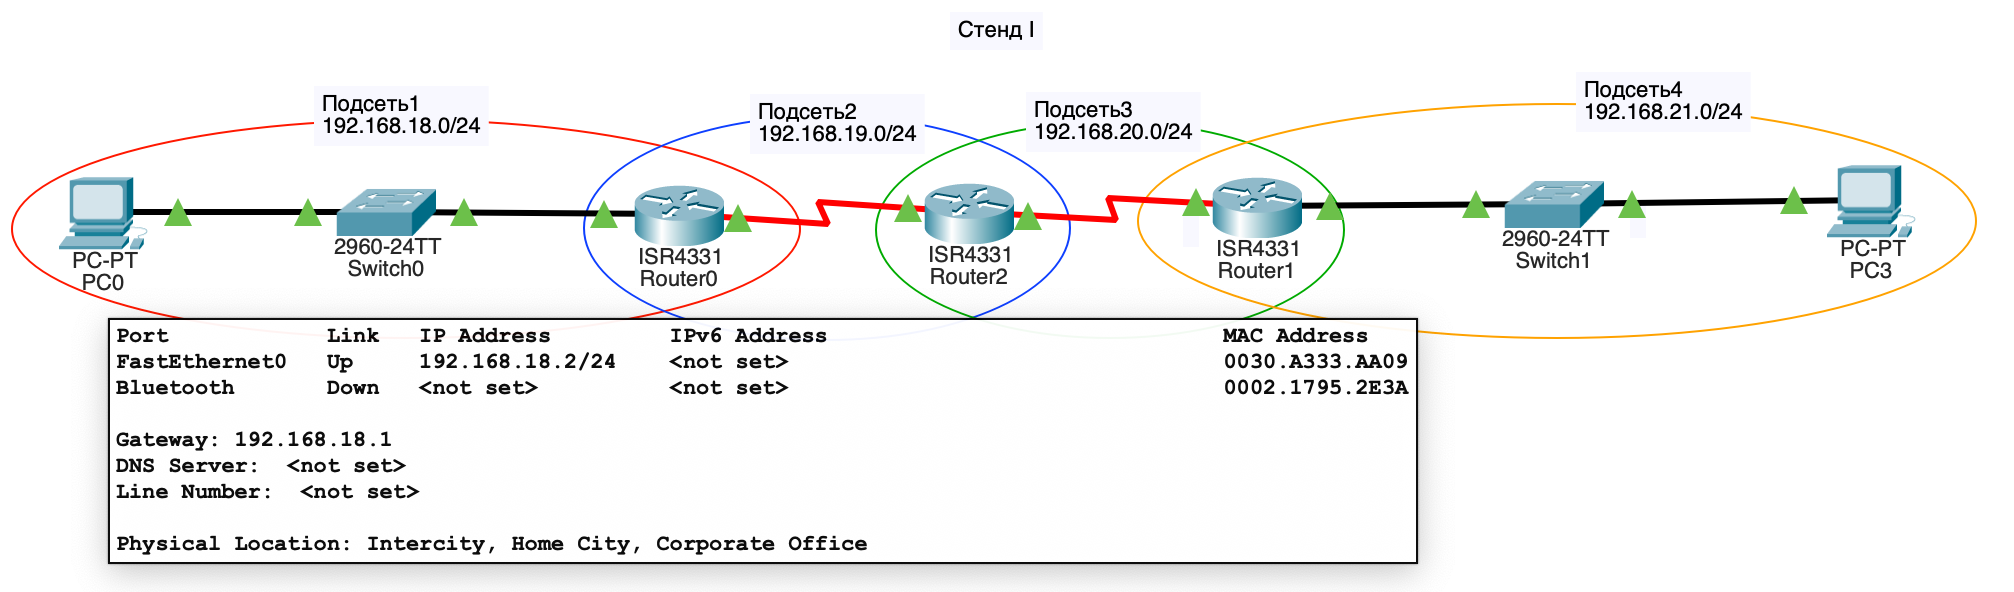
\includegraphics[scale=0.56]{1}
  \caption{Назначение адресов для стенда 1. }
\end{figure}

Назначение адресов для стенда 2 показано на рисунке 2, для примера показано, что компьютер 10 имеет IP адрес -- 192.168.21.2/24.

\begin{figure}[H]
  \centering
  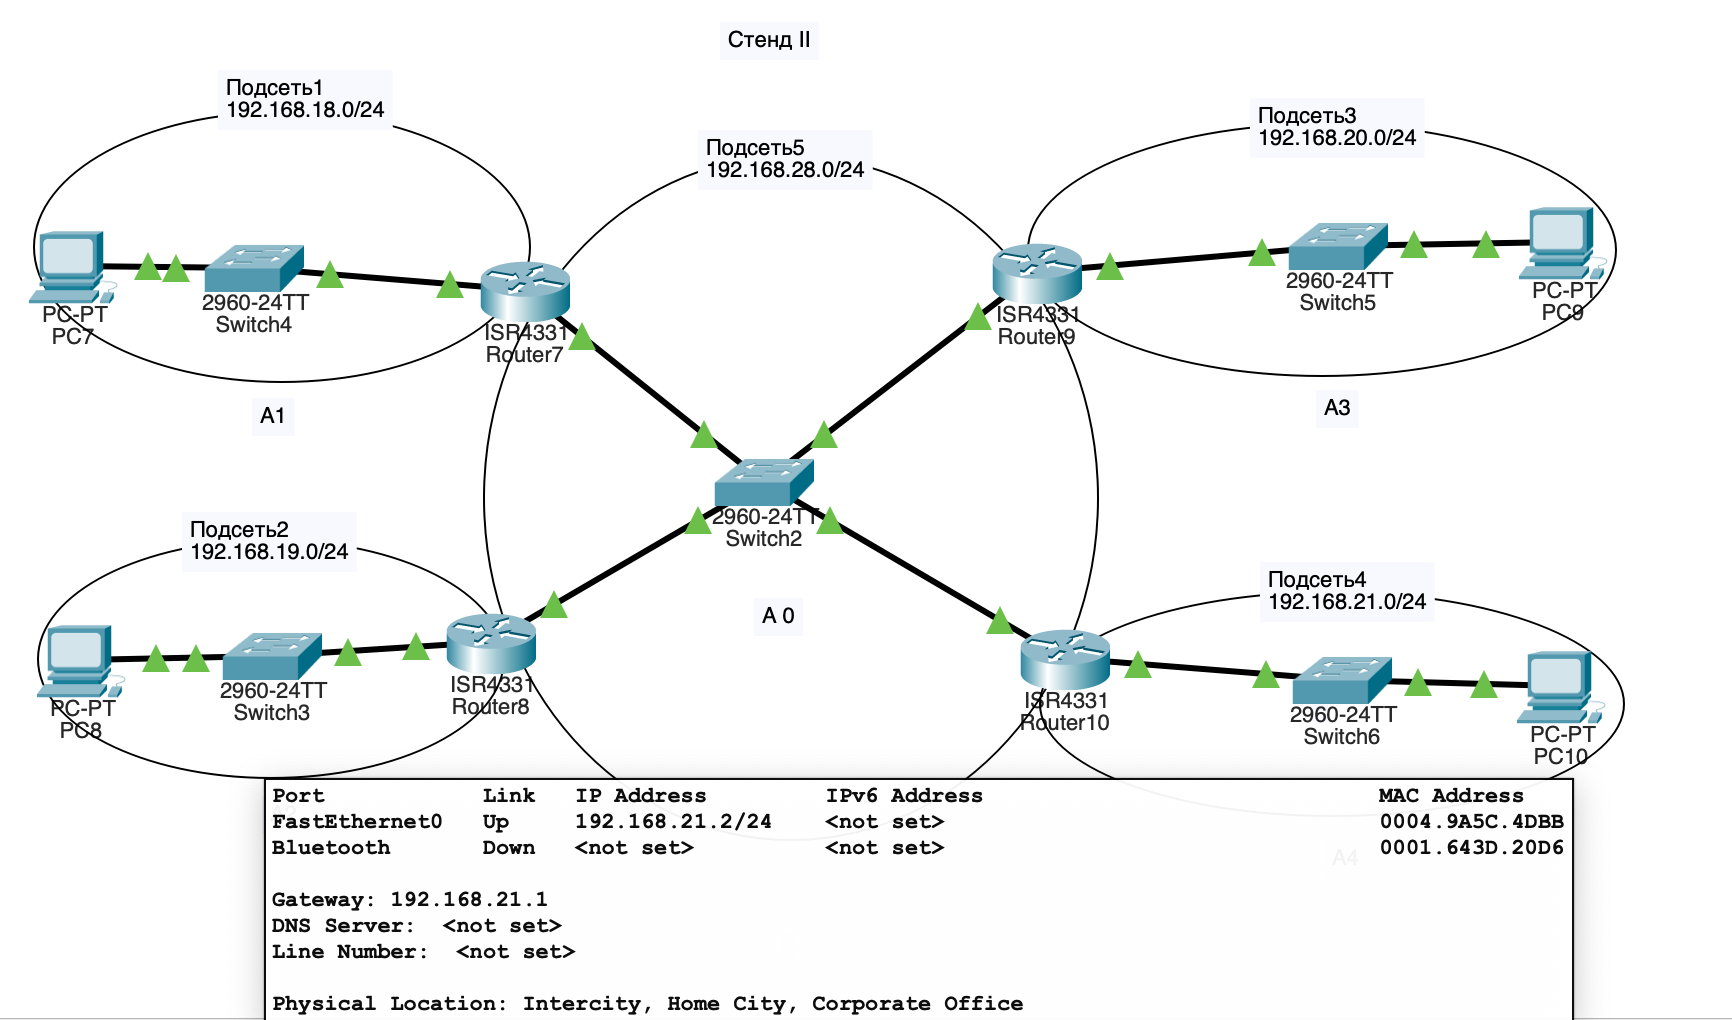
\includegraphics[scale=0.6]{2}
  \caption{Назначение адресов для стенда 2. }
\end{figure}

\item Настроить динамическую маршрутизацию в прилагаемом .pkt файле на стенде I через протокол RIPv2 так, чтобы пинг любым хостом или маршрутизатором любого другого хоста или маршрутизатора был успешным.

Настраиваем роутеры для использования RIPv2. 
 
\begin{figure}[H]
  \centering
  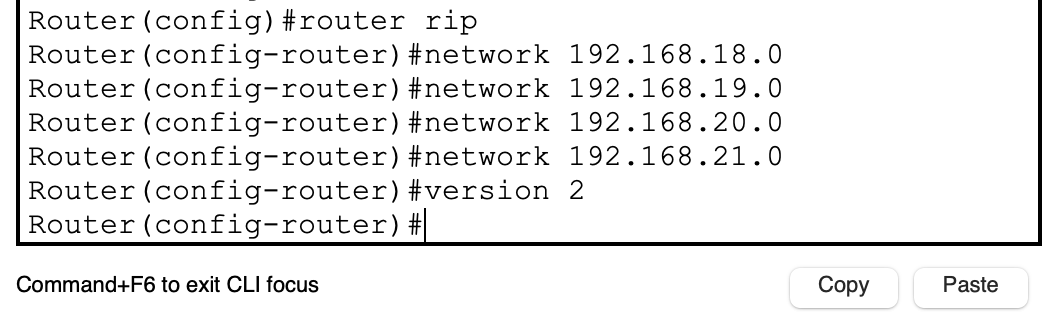
\includegraphics[scale=0.8]{3}
  \caption{Настройка роутеров. }
\end{figure}

Проверка информации протоколов маршрутизации, командой \textit{show ip protocols}.

\begin{figure}[H]
  \centering
  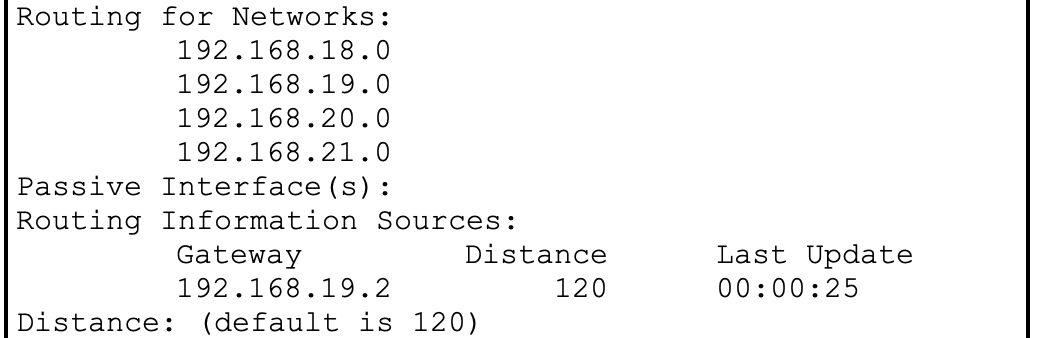
\includegraphics[scale=0.8]{4}
  \caption{Проверка протоколов маршрутизации. }
\end{figure}

На рисунке 5 представлен ping компьютером 3 компьютера 0, проверка работоспособности.

\begin{figure}[H]
  \centering
  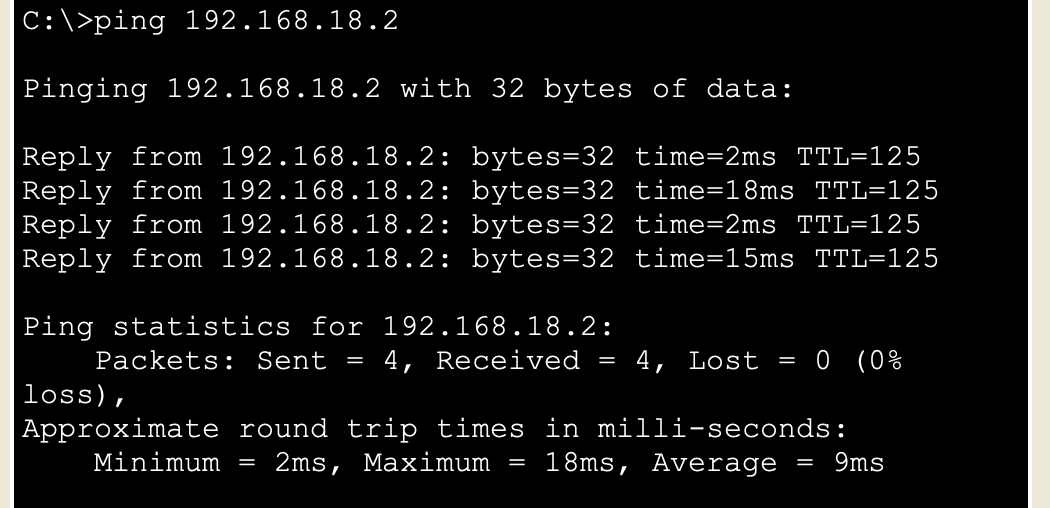
\includegraphics[scale=0.7]{5}
  \caption{Ping компьютером 3 компьютера 0. }
\end{figure}

\item Настроить динамическую маршрутизацию в сети в прилагаемом .pkt файле на стенде II через протокол OSPF так, чтобы пинг любым хостом или маршрутизатором любого другого хоста или маршрутизатора был успешным. Разделить при этом сеть на области OSPF в соответствии со схемой.  

Настройка роутеров для использования OSPF.

\begin{figure}[H]
  \centering
  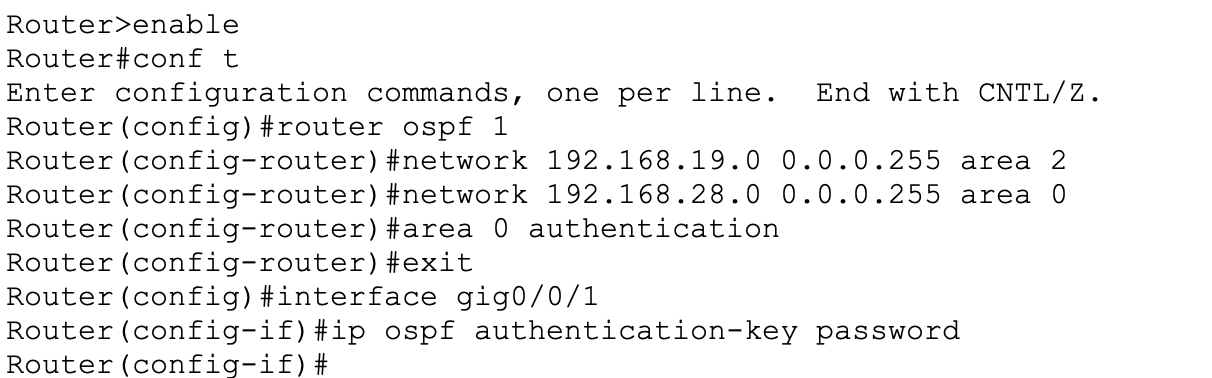
\includegraphics[scale=0.8]{6}
  \caption{Роутер 8. }
\end{figure}

\begin{figure}[H]
  \centering
  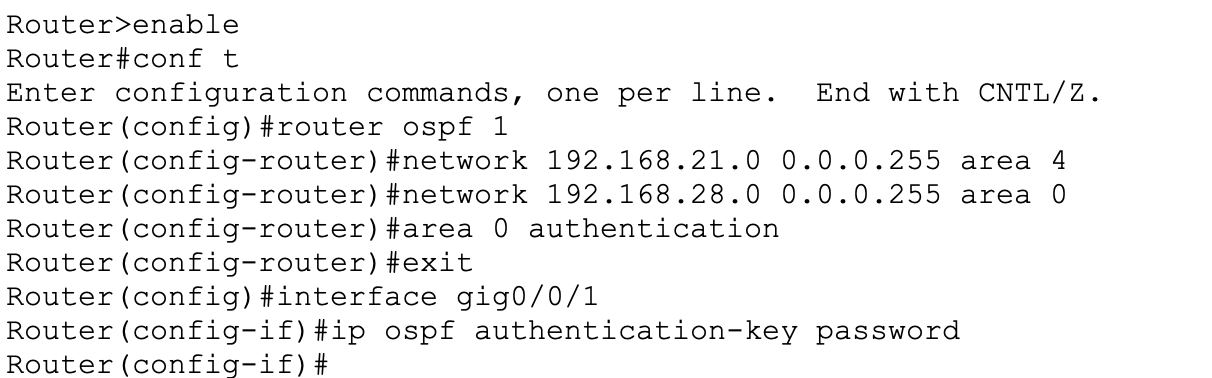
\includegraphics[scale=0.8]{7}
  \caption{Роутер 10. }
\end{figure}

Как видим список команд одинаков, отличается IP адрес сети и соотвественно номер области.

Для роутера 8 выведем информацию о статусе соседних устройств с помощью команды \textit{sh ip ospf neighbor}.

\begin{figure}[H]
  \centering
  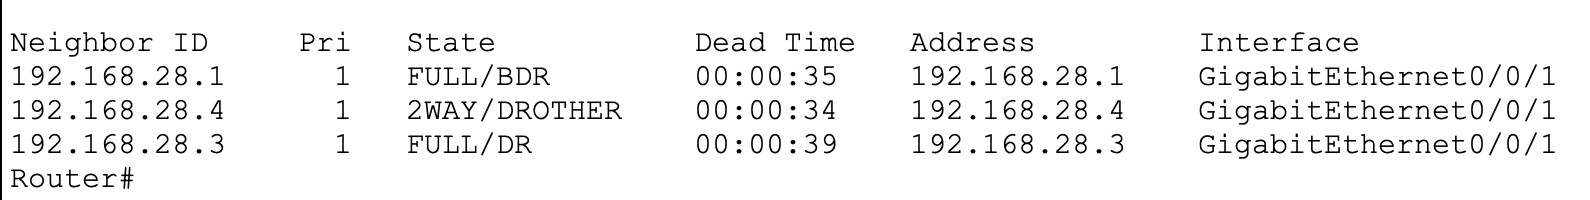
\includegraphics[scale=0.65]{8}
  \caption{Соседние устройства для роутера 8. }
\end{figure}

Роль BDR получил роутер роутер 7. DR получил роутер роутер 9.

Роль ABR имеют все роутеры, так как все они находятся на границе зон и соединяют их.

На рисунке 9 представлен ping компьютером 7 компьютера 10, проверка работоспособности.

\begin{figure}[H]
  \centering
  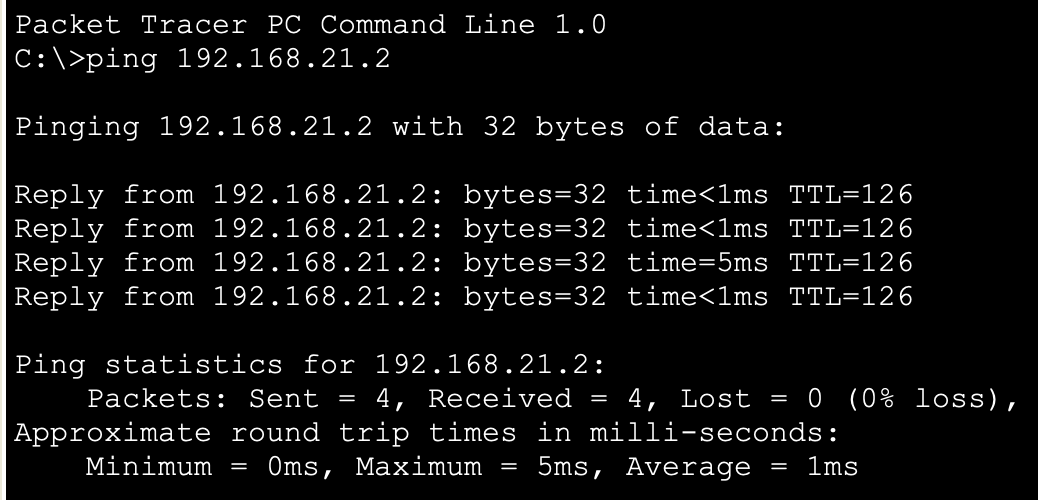
\includegraphics[scale=0.8]{9}
  \caption{Ping компьютером 7 компьютера 10. }
\end{figure}

\end{enumerate}


\end{document}